
\chapter{Wybrane metody tworzenia tablic sufiksów}

W~poniższym rozdziale omówione są wybrane metody tworzenia tablic sufiksów.
Algorytmy wybrane zostały na podstawie wyników testów wydajnościowych
zaprezentowanych w~pracach \cite{taxonomy} i~\cite{schurmann-phd} oraz
publikowanych na stronach [\ref{msufsort}] i~[\ref{mori-benchmark}].
Algorytmy uzyskujące dobre wyniki na dużych zbiorach danych -- szybkie \emph{w
praktyce} pochodzą z~rodziny algorytmów wykorzystujących \emph{polepszanie
wszerz}. W~poniższym zestawieniu opisane zostały również algorytmy
reprezentujące inne grupy metod tworzenia tablic sufiksów: \emph{polepszanie
wgłąb} i~\emph{sortowanie zredukowanych ciągów znaków}.


\section{Algorytm \emph{skew}}

Algorytm \emph{skew} został opracowany przez Petera Sandersa i~Juhę
K\"arkk\"ainena \cite{KS}. Dostępna jest
również implementacja tego algorytmu ich autorstwa [\ref{KScode}]. Opisywana
metoda pochodzi z~rodziny algorytmów wykorzystujących
\emph{sortowanie zredukowanych ciągów znaków}. 
Algorytm wykonuje 3 główne kroki:
\begin{enumerate}
  \item Tworzenie tablicy sufiksów zbudowanej z~sufiksów $S_i$ o~indeksach $i
  \bmod{3} \neq 0$. Problem jest redukowany do tworzenia tablicy sufiksów ciągu długości $2/3$ 
  rozmiaru ciągu wejściowego, a~następnie rozwiązywany rekurencyjne.
  \item Tworzenie tablicy sufiksów zbudowanej z~sufiksów pominiętych w~pierwszym kroku z~wykorzystaniem tablic sufiksów z~kroku 1.
  \item Połączenie zbudowanych tablic w~jedną.
\end{enumerate}

\noindent
Pierwszy (i najbardziej czasochłonny) krok algorytmu polega na posortowaniu
sufiksów $S_i$ dla $i \bmod{3} \neq 0$, czyli utworzeniu tablicy sufiksów
$\textit{SA}^{12}$. Jeżeli w~wyniku \emph{h-sortowania} dla $h=3$ wszystkie
grupy są jednoelementowe, to ten etap algorytmu się kończy. W~przeciwnym przypadku
każdemu sufiksowi $S_i$ nadawany jest identyfikator $x^{'}_i
\in [ 1, 2n/3]$ będący identyfikatorem jego \emph{3-grupy} powstałej po 
\emph{3-sortowaniu}. Następnie tworzony jest ciąg $x^{12} = [x^{'}_i : i
\bmod{3} = 1] \circ [x^{'}_i : i \bmod{3} = 2]$, którego tablica sufiksów
$\textit{SA}_{x^{12}}$ obliczana jest rekurencyjnie. Tablica $\textit{SA}^{12}$
wypełniana jest zgodnie z~poniższym wzorem ($n_1$ oznacza liczbę sufiksów o~etykietach $i$ takich, że $i \bmod{3} = 1$):  
\begin{displaymath}
\textit{SA}^{12}[i] = \left\{ 
    \begin{array}{l l}
    1 + 3k          & \textit{jeżeli } k = \textit{SA}_{x^{12}}[i] <  n_1, \\
    2 + 3(k - n_1)  & \textit{w przeciwnym wypadku}.
    \end{array} 
    \right.
\end{displaymath}

Drugi krok algorytmu polega na utworzeniu tablicy sufiksów $\textit{SA}^0$
złożonej z~sufiksów $S_i$, gdzie $i \bmod{3} = 0$. Tablica ta powstaje w~wyniku
sortowania par $(x[i], S_{i+1})$. Ponieważ porządek sufiksów $S_{i+1}$ jest
zawarty w~$\textit{SA}^{12}$, do znalezienia $\textit{SA}^0$ wystarczy posortować
stabilnie elementy $\textit{SA}^{12}[j]$ reprezentujące sufiksy
$\textit{SA}_{i+1}, i \bmod{3} = 0$ według wartości $x[i]$. Można tego dokonać
w~czasie liniowym jednym krokiem sortowania kubełkowego.

Trzeci krok algorytmu polega na połączeniu tablic $\textit{SA}^{12}$ i~$\textit{SA}^0$ w~jedną 
tablicę sufiksów. Porównywanie sufiksów $S_j$, gdzie $j\bmod{3}=0$ i~$S_i, i \bmod{3} \neq 0$ 
odbywa się na jeden z~dwóch sposobów:
\begin{itemize}
    \item Jeżeli $i \bmod{3} = 1$, to porządek sufiksów $S_i$ i~$S_j$ można
  ustalić porównując pary $(x[i], S_{i+1})$ oraz $(x[j], S_{j+1})$. Ponieważ $i+1
  \bmod{3} = 2$ i~$j+1 \bmod 3 = 1$ porządek sufiksów $S_{i+1}$ i~$S_{j+1}$
  można ustalić na podstawie ich pozycji w~$\textit{SA}_{x^{12}}$. Ta pozycja może
  być ustalana w~czasie stałym, jeżeli obliczona zostanie tablica
  $\textit{ISA}_{x^{12}}$.
  
    \item Analogicznie, jeżeli $i \bmod{3} =
  2$, to porównywane są trójki $(x[i], x[i+1], S_{i+2})$ i~$(x[j], x[j+1], S_{j+2})$, przy czym 
  sufiksy $S_{i+2}$ i~$S_{j+2}$ są zastępowane odpowiednimi wpisami z~tablicy  $\textit{ISA}_{x^{12}}$.
\end{itemize}


\begin{figure}[t]
        \begin{center} \small
            \begin{tabular}{r c c c c c c c c c c c c l}                           
                                  & 0  & 1    & 2    & 3  & 4    & 5     & 6  & 7    & 8    & 9  & 10   & 11            \\ \cmidrule{2-13} 
                 $x$ =          [ & b  & a    & d    & d  & a    & d     & d  & a    & c    & c  & a    & $\dollar$ & ] \\ 
$S_i, i \bmod{3} = 0$ =         [ & 0  &      &      & 3  &      &       & 6  &      &      & 9  &      &      & ]      \\ 
$S_i, i \bmod{3} \neq 0$ =      [ &    & 1    & 2    &    & 4    & 5     &    & 7    & 8    &    & 10   & 11   & ]      \\ 
$x[i..i+2], i\bmod{3} \neq 0$ = [ &    & add  & dda  &    & add  & dda   &    & acc  & cca  &    & a\$- & \$--  & ]     \\ \addlinespace[1em]

             \multicolumn{14}{c}{\emph{3-sortowanie} sufiksów o etykietach $i \bmod{3} \neq 0$ (wartości są indeksami po posortowaniu).} \\
                         $x'$ = [ &    & 3    & 5    &    & 3    & 5     &    & 2    & 4    &    & 1    & 0     & ]     \\ \addlinespace[1em]

             \multicolumn{14}{c}{Tworzenie ciągu $x^{12} = [x^{'}_i : i \bmod{3} = 1] \circ [x^{'}_i : i \bmod{3} = 2]$.} \\
                     $x^{12}$ = [ & 3  & 3    & 2    & 1  & 5    & 5     & 4  & 0    &  ] \\ \addlinespace[1em]

             \multicolumn{14}{c}{Obliczanie $\textit{SA}_{x^{12}}$ i $\textit{SA}^{12}$.} \\
       $\textit{SA}_{x^{12}}$ = [ & 7  & 3    & 2    & 1  & 0    & 6     & 5  & 4    &  ] \\ 
      $\textit{ISA}_{x^{12}}$ = [ & 4  & 3    & 2    & 1  & 7    & 6     & 5  & 0    &  ] \\ 
           $\textit{SA}^{12}$ = [ & 11 & 10   & 7    & 4  & 1    & 8     & 5  & 2    &  ] \\ \addlinespace[1em]

             \multicolumn{14}{c}{Sufiksy $S_i$, $i \bmod{3} = 1$ oraz $S_j$, $j = i - 1$ zgodnie z kolejnością w $\textit{SA}^{12}$.} \\
                        ~       [ & 10 & 7    & 4    & 1  & ] \\ 
                        ~       [ & 9  & 6    & 3    & 0  & ] \\ 
                       $x[j]$ = [ & c  & d    & d    & b  & ] \\ \addlinespace[1em]

             \multicolumn{14}{c}{Stabilne \emph{1-sortowanie} sufiksów $S_j$.} \\
              $\textit{SA}^0$ = [ & 0  & 9    & 6    & 3  & ] \\ \addlinespace[1em]

             \multicolumn{14}{c}{Scalanie tablic $\textit{SA}^0$ i $\textit{SA}^{12}$.} \\
                $\textit{SA}$ = [ & 11 & 10   & 7    & 4  & 1    &  0    & 9  & 8    &  6    & 3   &  5    &  2     & ] \\ 
            \end{tabular}            
        \end{center}                         
        \caption{Przykład tworzenia tablicy sufiksów według algorytmu \emph{skew}.
        Źródło: opracowanie własne.}%
        \label{rys:ks}
\end{figure}


\section{Algorytm \emph{qsufsort}}

Algorytm \emph{qsufsort} został przedstawiony w~pracy \cite{LS} autorstwa
Jespera Larrsona i~Kunihiko Sadakane. Autorzy pracę udostępniają również
implementację w~języku \texttt{C} [\ref{LScode}]. Opisywana metoda należy do
rodziny algorytmów wykonujących polepszanie wgłąb, opiera się na algorytmie
\emph{prefix-doubling}.

Sortowanie sufiksów wykonywane jest algorytmem \emph{ternary split
quicksort} \cite{bentley-sort}. Algorytm \emph{qsufsort} wykorzystuje
również twierdzenie opublikowane w~pracy \cite{karp}: dla obliczonych \SA{h} i~\ISA{h} posortowanie sufiksów $S_i$ według par (\ISA{h}$[i]$, \ISA{h}$[i+h]$),
$i+h \leq n$ tworzy \emph{2h-porządek} sufiksów, czyli
porządek według prefiksów długości $2h$.\footnote{Sufiksy $S_i, i > n - h$ są
zawsze w~pełni uporządkowane.}
Wynika to z~tego, że do ustalenia porządku sufiksów o~wspólnym prefiksie
długości $h$ wykorzystujemy porządek ich $\textit{h-następców}$, którzy są
również posortowani według h pierwszych znaków, co daje w~konsekwencji porządek
sufiksów według prefiksów długości $2h$.

Na początku działania algorytm wykonuje \emph{1-sort}, w~wyniku którego
powstają \SA{1} i~\ISA{1}. Numery grup w~odwróconej tablicy sufiksów
przypisywane są poprzez wybór ogona (pozycji ostatniego sufiksu w~tablicy
\SA{h}) danej grupy. Algorytm \emph{qsufsort} utrzymuje również tablicę $L$
długości $n$ używaną w~celu określania rozmiarów grup.
Wartość $L[j] = d$ oznacza, że grupa rozpoczynająca się na pozycji $j$ ma $d$
elementów. Wartości ujemne w~tablicy $L$ oznaczają ciągi jednoelementowych
grup (na przykład $-2$ oznacza dwie jednoelementowe grupy). 

Przeglądanie tablicy $L$ od lewej do prawej umożliwia omijanie grup
jednoelementowych w~procesie polepszania kubełków. Każda \emph{h-grupa}
sortowana jest osobno, jej sufiksy $S_i$ porównywane są na podstawie wartości
\ISA{h}$[i+h]$. Po posortowaniu wszystkich grup otrzymujemy \emph{2h-porządek}. 
Algorytm kończy swoje działanie, gdy wszystkie
{h-grupy} są jednoelementowe, czyli gdy $L[0] = -n$. W~przeciwnym wypadku $h$
jest podwajane, a~proces polepszania kubełków wykonywany po raz kolejny.

 \begin{figure}[t]
        \begin{center} \small
            \begin{tabular}{ r c c c c c c c c c c c c l}                           
                 & 0  & 1  & 2  & 3  & 4  & 5   & 6  & 7  & 8  & 9  & 10 & 11       \\\cmidrule{2-13} 
         $x$ = [ & a  & b  & e  & a  & c  & a   & d  & a  & b  & e  & a  &
         $\dollar$ & ] \\ \SA{1} = [ & 11 & (0 & 3  & 5  & 7  & 10) & (1 & 8) & 4  & 6  & (2 & 9)   & ] \\ 
     \ISA{1} = [ & 5  & 7  & 11 & 5  & 8  &  5  & 9  & 5  & 7  & 11 & 5  & 0    &] \\ 
	$L$  = [ & -1 & 5  &    &    &    &     & 2  &    & -2 &    & 2  &      &] \\ \cmidrule{2-13}
      \SA{2} = [ & 11 & 10 & (0 & 7) & 3  & 5   & (1 & 8) & 4  & 6  & (2 & 9)   & ] \\ 
     \ISA{2} = [ & 3  & 7  & 11 & 4  & 8  & 5   & 9  & 3  & 7  & 11 & 2  & 0    &] \\ 
	$L$  = [ & -2 &    & 2  &    & -2 &     & 2  &    & -2 &    & 2  &      &] \\ \cmidrule{2-13}
      \SA{4} = [ & 11 & 10 & (0 & 7) & 3  & 5   & 8  & 1  & 4  & 6  & 9  & 2   & ] \\ 
     \ISA{4} = [ & 3  & 7  & 11 & 4  & 8  & 5   & 9  & 3  & 6  & 10 & 1  & 0    &] \\ 
	$L$  = [ & -2 &    & 2  &    & -8 &     &    &    &    &    &    &      &] \\ \cmidrule{2-13}
      \SA{8} = [ & 11 & 10 & 7  & 0  & 3  & 5   & 8  & 1  & 4  & 6  & 9  & 2   & ] \\ 
     \ISA{8} = [ & 3  & 7  & 11 & 4  & 8  & 5   & 9  & 2  & 6  & 10 & 1  & 0    &] \\ 
	$L$  = [ & -12 &   &    &    &    &     &    &    &    &    &    &      &] \\ 

            \end{tabular}            
        \end{center}                         
    \caption{Przebieg algorytmu \emph{qsufsort} dla słowa ,,abeacadabea''.
    Źródło: opracowanie własne na podstawie \cite{taxonomy}.}%
    \label{rys:ls}
    \end{figure}

Algorytm \emph{qsufsort} da się optymalizować pod kątem redukcji zużycia
pamięci. Możliwe jest kompletne wyeliminowanie tablicy $L$. Do wyznaczania \emph{h-grup} zawierających więcej niż 1 element można wykorzystać tablicę
\ISA{}, rozmiar grupy wyznacza się wtedy na podstawie jej pierwszego elementu.
Jeżeli $j$ oznacza pozycję pierwszego elementu grupy w~\SA{}, a~$i=$\SA{h}$[j]$, to jej rozmiar wynosi \ISA{h}$[i] - j + 1$.
Złożoność pamięciowa algorytmu może również zostać zredukowana poprzez
nadpisanie ciągu wejściowego i~wykorzystanie tego obszaru pamięci do
przechowywania \ISA{} po obliczeniu \SA{1}.


\section{Algorytm \emph{deep shallow}}

Algorytm \emph{deep shallow} jest rozwinięciem algorytmu \emph{copy}
opracowanym przez Paolo Ferraginę i~Giovanniego Manziniego. Opublikowany został
w~pracy \cite{MF}. Kod algorytmu w~języku \texttt{C} dostępny jest pod adresem
[\ref{MFcode}], jego autorem jest Giovanni Manzini.

Pierwszym krokiem algorytmu jest uporządkowanie sufiksów według dwóch
pierwszych znaków (\emph{2-sortowanie}). Każdy z~utworzonych w~ten
sposób kubełków sortowany jest algorytmem \emph{multikey quicksort}
\cite{bentley}, który jest przerywany po osiągnięciu poziomu rekurencji równemu
$L$, czyli jeżeli wewnątrz kubełka istnieje grupa sufiksów o~wspólnym prefiksie
długości $L$. Podejście to nosi nazwę sortowania płytkiego (\english{shallow
sorting}).

Sortowanie znajdowanych sufiksów o~wspólnym prefiksie długości $L$
nazwane zostało przez autorów algorytmu \emph{deep shallow} sortowaniem
głębokim (\english{deep sort}). Przebieg działania głębokiego sortowania zależy
od wielkości zbioru sortowanych sufiksów. Jeżeli liczność zbioru nie przekracza
zadanej wartości $B$, to sufiksy są sortowane algorytmem \emph{blind sort}. W~przeciwnym przypadku do posortowania sufiksów wykorzystane zostanie zmodyfikowany algorytm
\emph{ternary split quicksort} \cite{bentley-sort}. Autorzy sugerują użycie
wartości $B = n \times 0.0005$ jako progu wielkości zbioru.

Algorytm \emph{blind sort} opiera swoje działanie na strukturze danych
nazywanej \definicja{blind trie} \cite{btree}, która jest typem skompresowanego
drzewa którego węzły wewnętrzne przechowują liczby określające długość wspólnego
prefiksu węzłów potomnych (jeżeli węzeł zawiera liczbę $k$, to jego węzły
potomne różnią się na pozycji $k+1$). Przykładowe drzewo \emph{blind trie}
znajduje się na rysunku \ref{rys:blind-trie}. 

Algorytm \emph{blind sort} tworzy drzewo \emph{blind trie}, a~następnie
przegląda je od lewej do prawej uzyskując w~ten sposób porządek leksykograficzny
sekwencji podanych na wejściu (w drzewie \emph{blind trie} węzły potomne danego
węzła są uporządkowane). Poważną wadą metody \emph{blind sort} jest jej
złożoność pamięciowa, sięgająca nawet $36m$, gdzie $m$ oznacza liczbę ciągów do
posortowania.

\begin{figure}[t]
    \begin{center}
       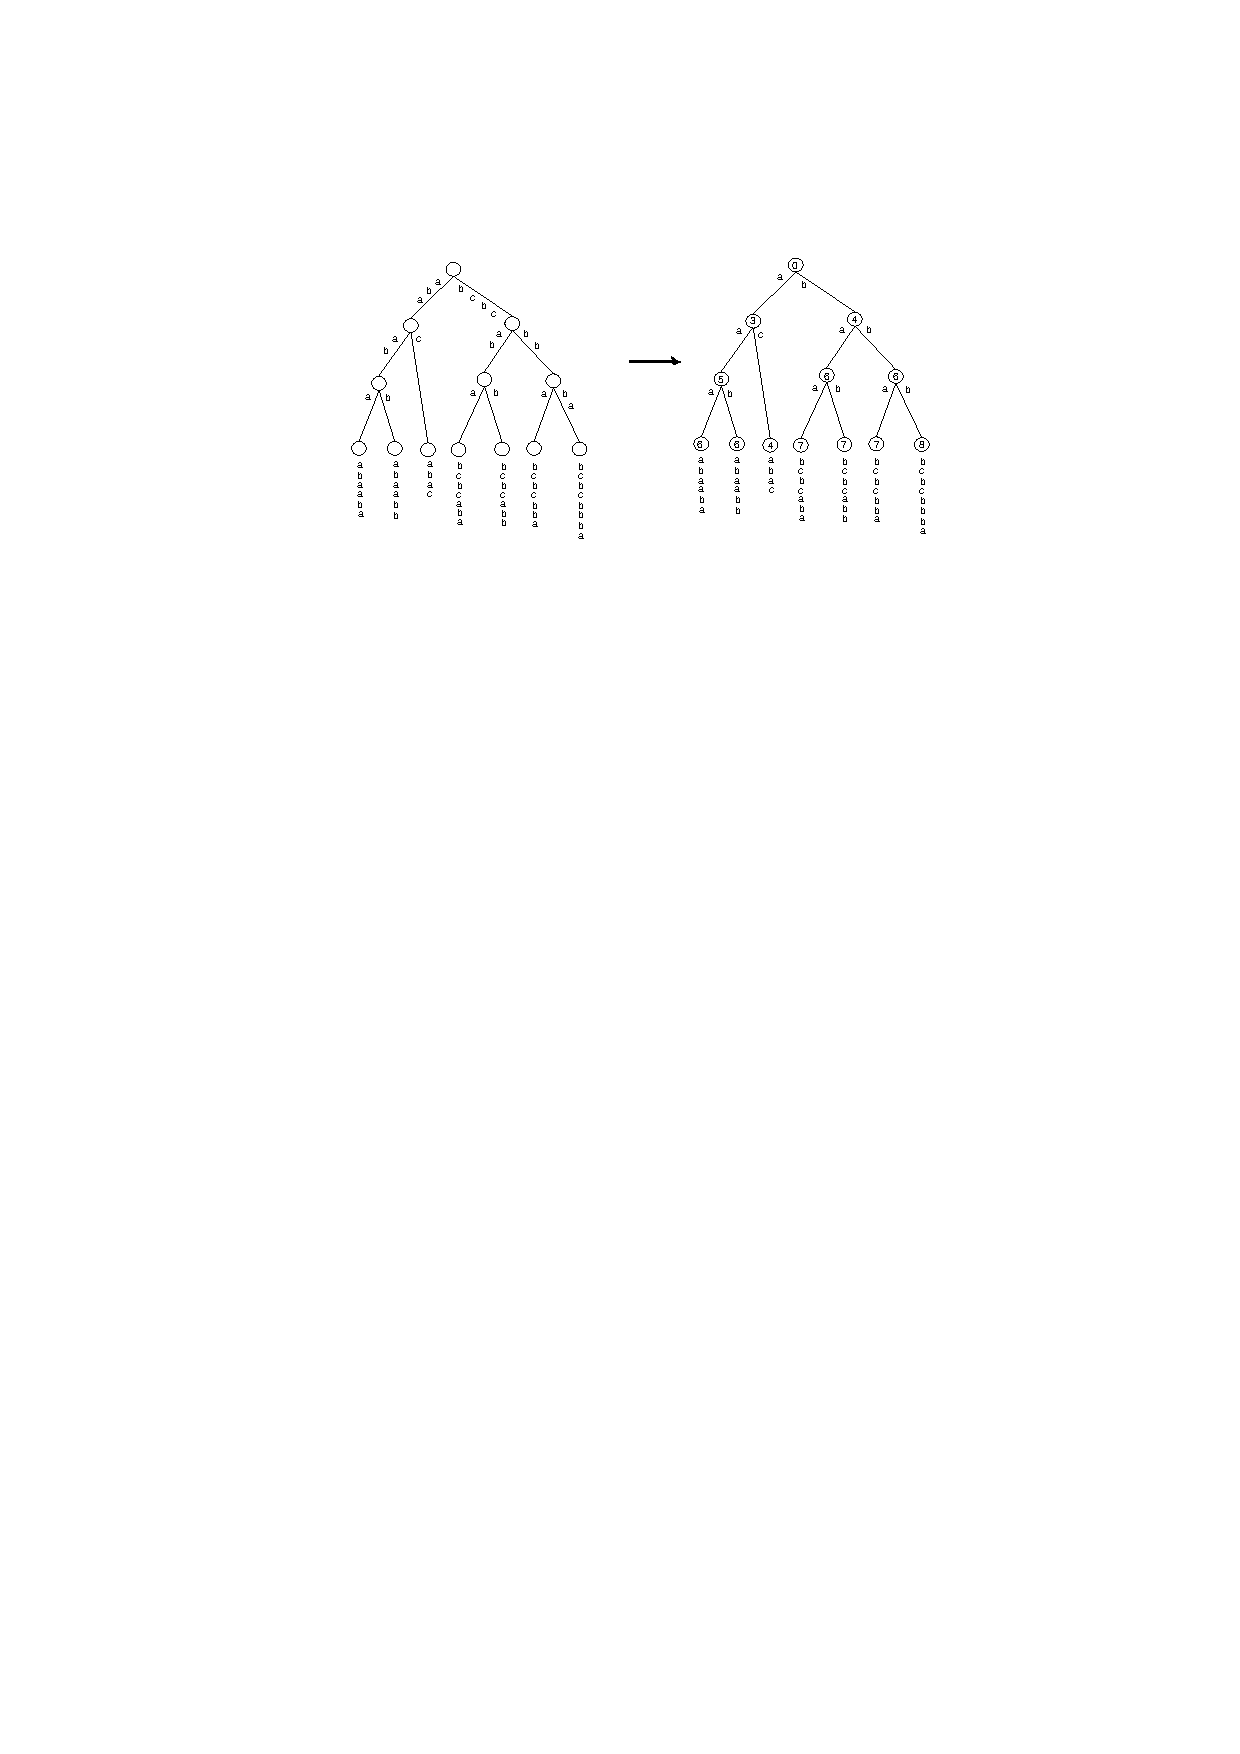
\includegraphics[width=.9\linewidth]{figures/blindtrie.pdf}
    \end{center}
    \caption{Drzewo skompresowane oraz odpowiadające mu drzewo \emph{blind trie}
    zbudowane na zbiorze sekwencji \emph{abaaba, abaabb, abac, bcbcaba, bcbcabb, bcbcbba, bcbcbbba}. 
    Źródło: \cite{MF}.}\label{rys:blind-trie}
\end{figure}

Do sortowania zbiorów większych niż $B$ autorzy algorytmu \emph{deep shallow}
użyli zmodyfikowanego algorytmu \emph{ternary split quicksort}, opisanego w~pracy \cite{bentley-sort}. Dokonali oni następujących zmian:
\begin{enumerate}
  \item Jeżeli na dowolnym etapie rekursji zbiór sufiksów jest mniejszy niż
  $B$, to do jego sortowania użyty zostaje algorytm \emph{blind sort}.
  \item Podczas fazy podziału sufiksów obliczane są $L_S$ i~$L_L$, czyli
  długość najdłuższego wspólnego prefiksu elementu osiowego (\english{pivot}) i~zbioru elementów mniejszych ($L_S$) oraz większych ($L_L$) od elementu
  osiowego. Dzięki temu podczas sortowania sufiksów w~tych zbiorach można
  pomijać prefiksy długości $L_S$ lub $L_L$.
\end{enumerate}

Paolo Ferragina i~Giovanni Manzini w~pracy \cite{MF} wymieniają trzy zalety
dwuetapowego podejścia do problemu sortowania sufiksów zastosowanego w~algorytmie \emph{deep shallow}:
\begin{enumerate}
  \item Szybkie wykrywanie grup sufiksów o~długim wspólnym prefiksie.
  \item Rozmiar stosu użytego podczas rekurencji w~fazie sortowania płytkiego
  jest ograniczony parametrem $L$ i~nie zależy od rozmiaru wejścia.
  \item Jeżeli długość najdłuższego wspólnego prefiksu sufiksów jednego kubełka
  nie przekracza $L$, to uporządkowywane są one efektywnym algorytmem
  sortowania ciągu znaków (\emph{multikey quicksort}).
\end{enumerate}
 
 
\section{Algorytm \emph{two-stage}}

Hideo Itoh i~Hozumi Tanaka zaproponowali w~pracy \cite{IT} algorytm tworzenia
tablic sufiksów o~nazwie \emph{two-stage}. Algorytm ten dzieli sufiksy na dwie
kategorie: sufiksy typu $A$ to wszystkie sufiksy $S_i$ spełniające nierówność $x[i] > x[i+1]$,
sufiksy typu $B$ to sufiksy spełniające nierówność $x[i] \leq x[i+1]$.
 
Algorytm rozpoczyna swoje działanie od obliczenia \SA{1}. Początek i~koniec
każdej grupy zapamiętywany jest w~tablicach $\mathit{head}$ i~$\mathit{tail}$. Długość tych tablic odpowiada wielkości słownika symboli.
Sufiksy w~każdej \emph{1-grupie} są uporządkowywane w~taki sposób, żeby sufiksy typu $A$
były przed sufiksami typu $B$. Wynika to z~tego, że jeżeli sufiksy $S_i$ typu $A$ i~$S_j$ typu $B$ mają wspólny prefiks długości jednego symbolu, to sufiks $S_i$ poprzedza sufiks $S_j$ w~porządku leksykograficznym. Indeksy pierwszych sufiksów typu $B$ każdej
grupy zapamiętywane są w~tablicy $\mathit{part}$ długości $\sigma$.
Kolejnym krokiem algorytmu jest sortowanie sufiksów typu $B$ wewnątrz każdej
grupy. Autorzy pracy \cite{IT} sugerują użycie do tego celu algorytmu
\cite{bentley}, nie jest to jednak konieczne i~można do tego celu użyć innego
algorytmu sortowania ciągów znaków. 


Następnie ustalany jest porządek sufiksów typu $A$. Tablica \SA{} przeglądana
jest od lewej do prawej, znajdując wartości $i=\mathit{SA}[j], j=0,1,\ldots,n-1$. Jeżeli
$S_{i-1}$ jest jeszcze nieuporządkowanym sufiksem typu $A$, to umieszczany jest
na początku grupy do której należy. Odpowiednia wartość w~tablicy \emph{head} jest potem
inkrementowana. Po jednokrotnym przejrzeniu \SA{} sufiksy są już w~pełni
posortowane, co kończy algorytm (przykład na rysunku~\ref{rys:it}).

\begin{figure}[ht]
        \begin{center} \small
            \begin{tabular}{r c c c c c c c c c c c c l}                           
                 & 0  & 1  & 2  & 3  & 4  & 5   & 6  & 7  & 8  & 9  & 10 & 11       \\ \cmidrule{2-13} 
         $x$ = [ & b  & a  & d  & d  & a  & d   & d  & a  & c  & c  & a  &
         $\dollar$ & ] \\ type = [ & A  & B  & B  & A  & B  & B   & A  & B  & B  & A  & A  & B    & ] \\ \addlinespace[1em]
	
       \multicolumn{14}{c}{\emph{1-sort}}\\
       \SA{} = [ & 11 & (-- & 1  & 4  & 7) & (--) & (-- & 8) & (-- & --  & 2  & 5)   & ] \\
        type = [ & B  & A  & B  & B  & B  & A   & A  & B  & A  & A  & B  & B    & ] \\ \addlinespace[1em]
	
       \multicolumn{14}{c}{sortowanie sufiksów typu $B$} \\
       \SA{} = [ & 11 & (-- & 7  & 4  & 1) & (--) & (-- & 8) & (-- & --  & 5  & 2)   & ] \\ \addlinespace[1em]
	
       \multicolumn{14}{c}{wstawianie sufiksów typu $A$}\\
       \SA{} = [ & 11 & 10 & 7  & 4  & 1  & --   & --  & 8  & --  & --  & 5  & 2   & ] \\
       \SA{} = [ & 11 & 10 & 7  & 4  & 1  & --   & 9  & 8  & --  & --  & 5  & 2   & ] \\
       \SA{} = [ & 11 & 10 & 7  & 4  & 1  & --   & 9  & 8  & 6  & --  & 5  & 2   & ] \\
       \SA{} = [ & 11 & 10 & 7  & 4  & 1  & --   & 9  & 8  & 6  & 3  & 5  & 2   & ] \\
       \SA{} = [ & 11 & 10 & 7  & 4  & 1  & 0   & 9  & 8  & 6  & 3  & 5  & 2   & ] \\
            \end{tabular}            
        \end{center}                         
    \caption{Przebieg algorytmu \emph{two-stage} dla słowa ,,baddaddacca''.
    Nieuporządkowane sufiksy typu $A$ oznaczane są znakiem ,,--''. Źródło:
    opracowanie własne na podstawie \cite{taxonomy}.}%
    \label{rys:it}
\end{figure}


\section{Algorytm \emph{improved two-stage}}

Algorytm \emph{improved two-stage} opisany został w~pracy \cite{MP}, której
autorami są Simon Puglisi i~Michael Maniscalco.
Kwestia autorstwa tego algorytmu pozostaje niejasna, metoda ta posiada aż trzy niezależne
implementacje powstałe przed publikacją artykułu:
\begin{itemize}
	\item \emph{archon } [\ref{archon}] autorstwa Dimy Małyszewa,
	\item \emph{divsufsort} [\ref{libdivsufsort}] której autorem jest Yuta Mori,
	\item \emph{msufsort} [\ref{msufsort}] autorstwa Michaela Maniscalco.
\end{itemize}
Wymienione implementacje algorytmu \emph{improved two-stage} napisane zostały w~języku \texttt{C++}. 

Na początku sufiksy są dzielone na dwie kategorie: sufiksy typu $A$ to sufiksy
$S_i$ spełniające nierówność $S_i > S_{i+1}$, sufiksy typu $B$ to sufiksy
spełniające nierówność $S_i \leq S_{i+1}$. Sufiks o~identyfikatorze $n-1$ należy
do obu grup. Następnie, sufiksy $S_i$ typu $B$ których następny sufiks $S_{i+1}$ jest typu $A$ oznaczane są jako
sufiksy typu $B^*$. 

Kolejnym krokiem algorytmu jest znalezienie granic grup które powstałyby po
\emph{2-sortowaniu}. Następnie tworzony jest \emph{2-porządek} sufiksów typu
$B^*$. \emph{2-sortowanie} wszystkich sufiksów nie jest konieczne w~tym
momencie, a~jego pominięcie zmniejsza czas działania algorytmu.
Sufiksy typu $B^*$ należące do jednej grupy są sortowane zgodnie z~metodami
przedstawionymi w~pracach \cite{bentley, MF} i~umieszczane na początkowych
pozycjach wewnątrz kubełka w~tablicy \SA{}. 

Porządek sufiksów typu $B$ ustalany jest poprzez przeglądanie tablicy \SA{} od
prawej do lewej. Dla każdego sufiksu $\mathit{SA}[i]$ odczytanego podczas
przeglądania tablicy sufiks $\mathit{SA}[i]-1$ jest wstawiany na ostatnią pustą
pozycję wewnątrz swojej grupy jeżeli jest sufiksem typu $B$.

Wstawianie sufiksów typu $A$ wykonywane jest w~sposób identyczny jak w~algorytmie
\emph{two-stage} (przykład przedstawiono na rysunku \ref{rys:div}).

\begin{figure}[t]
        \begin{center}\small  
            \begin{tabular}{r c c c c c c c c c c c c c c l}                           
                 & 0   & 1  & 2   & 3      & 4  & 5 & 6  & 7      & 8   & 9  & 10 & 11    & 12  & 13      \\\cmidrule{2-15} 
         $x$ = [ & e   & d  & a   & b      & d  & c & c  & d      & e   & e  &
         d  & a     & b   & $\dollar$ & ] \\ type = [ & A   & A  & B   & $B^*$  & A  & B & B  & $B^*$  & A   & A  & A  & $B^*$ & A   &      &  ] \\ \addlinespace[1em]
	\multicolumn{16}{c}{Obliczanie wielkości \emph{2-grup}}\\
      \SA{2} = [ & --  & (-- & --) & --     & --  & -- & --  & (--     & --) & --  & -- & (--    & --)  & --    & ] \\ \addlinespace[1em]
    \multicolumn{16}{c}{Sortowanie sufiksów typu $B^*$} \\
       \SA{} = [ & --   & 11 & --   & --      & 3  & -- & --  & --      & --   & --  & 7  & --     & --   & --    & ] \\ \addlinespace[1em]  
	\multicolumn{16}{c}{Wstawianie sufiksów typu B}\\
       \SA{} = [ & --   & 11 & --   & --      & 3  & -- & 6  & --      & --   & --  & 7  & --     & --   & --    & ] \\  
       \SA{} = [ & --   & 11 & --   & --      & 3  & 5 & 6  & --      & --   & --  & 7  & --     & --   & --    & ] \\  
       \SA{} = [ & --   & 11 & 2   & --      & 3  & 5 & 6  & --      & --   & --  & 7  & --     & --   & --    & ] \\ \addlinespace[1em]
	\multicolumn{16}{c}{Wstawianie sufiksów typu A}\\
       \SA{} = [ & 13  & 11 & 2   & --      & 3  & 5 & 6  & --      & --   & --  & 7  & --     & --   & --    & ] \\  
       \SA{} = [ & 13  & 11 & 2   & 12     & 3  & 5 & 6  & --      & --   & --  & 7  & --     & --   & --    & ] \\  
       \SA{} = [ & 13  & 11 & 2   & 12     & 3  & 5 & 6  & 10     & --   & --  & 7  & --     & --   & --    & ] \\  
       \SA{} = [ & 13  & 11 & 2   & 12     & 3  & 5 & 6  & 10     & 1   & --  & 7  & --     & --   & --    & ] \\  
       \SA{} = [ & 13  & 11 & 2   & 12     & 3  & 5 & 6  & 10     & 1   & 4  & 7  & --     & --   & --    & ] \\  
       \SA{} = [ & 13  & 11 & 2   & 12     & 3  & 5 & 6  & 10     & 1   & 4  & 7  & 9     & --   & --    & ] \\  
       \SA{} = [ & 13  & 11 & 2   & 12     & 3  & 5 & 6  & 10     & 1   & 4  & 7  & 9     & 0   & --    & ] \\  
       \SA{} = [ & 13  & 11 & 2   & 12     & 3  & 5 & 6  & 10     & 1   & 4  & 7  & 9     & 0   & 8    & ] \\  
            \end{tabular}            
        \end{center}                         
    \caption{Przebieg algorytmu \emph{divsufsort} dla słowa ,,edabdccdeedab''.
 			Źródło: opracowanie własne na podstawie \cite{div}.}%
    \label{rys:div}
\end{figure}


\section{Algorytm \emph{bpr}}

Klaus-Bernd Schürmann w~pracy \cite{schurmann-phd} zaproponował algorytm
\emph{bpr} (\emph{bucket pointer refinement}, polepszanie wskaźników na
kubełki). Algorytm ten jest poprawioną wersją metody przedstawionej w~pracy
\cite{bpr-old} napisanej przez Klausa-Bernda Schürmanna i~Jensa Stoye. Kod
algorytmu \emph{bpr} w~języku \texttt{C++} dostępny jest na stronie [\ref{bpr-code}].

Pierwszym krokiem algorytmu jest posortowanie sufiksów według $q$-pierwszych
znaków, czyli \emph{q-sortowanie}. Wartość parametru $q$ obliczana jest na
podstawie liczby różnych symboli (czyli wielkości alfabetu) w~ciągu wejściowym, jej wartość maleje wraz ze
wzrostem wielkości słownika sekwencji wejściowej. Następnie obliczana jest
przybliżona odwrotna tablica sufiksów \ISA{} (kubełki identyfikowane są pozycją
ich ostatniego elementu w~przybliżonej tablicy sufiksów), nazywana w~pracy
\cite{schurmann-phd} \emph{tablicą wskaźników na kubełki}.

Algorytm \emph{bpr} działa według schematu \emph{polepszania kubełków wgłąb} i~korzysta z~techniki \emph{pull}. Sufiksy $S_i$ i~$S_j$ należące
do jednej \emph{h-grupy} porównywane są poprzez porównanie wartości
\ISA{}$[h + i]$ i~\ISA{}$[h + j]$.

Każda ze znalezionych na początku grup sortowana jest algorytmem \emph{ternary
split quicksort} \cite{bentley-sort}. Parametr $h$ przyjmuje początkowo
wartość $q$. Algorytm ten wybiera jeden z~sufiksów danej grupy jako element
osiowy (\english{pivot}) $S_p$ o~wartości klucza $K_p = \textit{ISA}[h + p]$. Sufiksy danej grupy dzielone są na trzy
podgrupy: sufiksy o~wartości klucza mniejszej, równej lub większej niż $K_p$.
Każda z~tych podgrup jest następnie w~ten sam sposób sortowana, przy czym
dla grupy sufiksów o~wartości klucza równej elementowi osiowemu wartość
parametru $h$ zwiększana jest o~$q$, ponieważ wszystkie jej sufiksy mają
wspólny prefiks długości $h + q$. Wynika to z~tego, że elementy kubełka o~wspólnym prefiksie długości $h$ sortowane są na podstawie pozycji ich
\emph{h-następników}, dla których nie znamy długości wspólnego prefiksu.
Wiadomo tylko tyle, że były posortowane na początku działania algorytmu według
$q$ pierwszych znaków. Podobnie jak w~algorytmie \emph{qsufsort}, równa wartość
klucza $\textit{ISA}[h + i]$ i~$\textit{ISA}[h + j]$ oznacza że sufiksy $S_i$ i~$S_j$ mają wspólny prefiks długości $h+q$. Fundamentalna różnica między
algorytmami \emph{bpr} i~\emph{qsufsort} polega na tym, że pierwszy z~nich
realizuje schemat \emph{polepszania kubełków wgłąb}, a~drugi \emph{polepszania
wszerz}. Dzięki temu, algorytm \emph{qsufsort} w~kolejnej iteracji może
podwajać wartość parametru $h$.

Istotną cechą algorytmu \emph{bpr} jest to, że po każdym podziale grupy na
podgrupy wykonywana jest aktualizacja wpisów w~tablicy \ISA{} odpowiadających
jej elementom, zgodnie ze wzorem $\textit{ISA}[i] =$ \emph{pozycja
ostatniego elementu podgrupy}. Na rysunku \ref{rys:bpr} przedstawiony został
przebieg działania algorytmu \emph{bpr} na przykładzie ciągu ,,DEBDEBDEA''.

\begin{figure}[t]
    \begin{center}\small
    \begin{tabular}{r c c c c c c c c c l}
                     &  0   &      1      &      2      &      3      &     4      &      5      &     6      &      7      &      8      &     \\ \cmidrule{2-10} 
               $x=[$ &  D   &      E      &      B      &      D      &     E      &      B      &     D      &      E      &      A      & ]   \\ \addlinespace[.5em] 
                                                  \multicolumn{11}{c}{Podział na kubełki, $q=2$}                                                \\ 
                     &  A   &  \multicolumn{2}{c}{BD}   &         \multicolumn{3}{c}{DE}         &     EA     &  \multicolumn{2}{c}{EB}   &     \\ 
     $\textit{SA}=[$ &  8   & \textbf{(2} & \textbf{5)} &     (0      &     3      &     6)      &     7      &     (1      &     4)      & $]$ \\ 
    $\textit{ISA}=[$ &  5   &      8      &      2      &      5      & \textbf{8} &      2      &     5      & \textbf{6}  &      0      & $]$ \\ \addlinespace[.5em] 
                                                  \multicolumn{11}{c}{Po posortowaniu kubełka BD}                                               \\ 
     $\textit{SA}=[$ &  8   &      5      &      2      & \textbf{(0} & \textbf{3} & \textbf{6)} &     7      &     (1      &     4)      & $]$ \\ 
    $\textit{ISA}=[$ &  5   &      8      & \textbf{2}  &      5      &     8      & \textbf{1}  &     5      &      6      & \textbf{0}  & $]$ \\ \addlinespace[.5em] 
                                                  \multicolumn{11}{c}{Po posortowaniu kubełka DE}                                               \\ 
     $\textit{SA}=[$ &  8   &      5      &      2      &      6      &     3      &      0      &     7      & \textbf{(1} & \textbf{4)} & $]$ \\ 
    $\textit{ISA}=[$ &  5   &      8      &      2      & \textbf{4}  &     8      &      1      & \textbf{3} &      6      &      0      & $]$ \\ \addlinespace[.5em] 
                                         \multicolumn{11}{c}{Po posortowaniu kubełka EB, koniec algorytmu}                                      \\ 
     $\textit{SA}=[$ &  8   &      5      &      2      &      6      &     3      &      0      &     7      &      4      &      1      & $]$ \\ 
    $\textit{ISA}=[$ &  5   &      8      &      2      &      4      &     7      &      1      &     3      &      6      &      0      & $]$ \\ 
    \end{tabular}
    \end{center}

    \caption{Przebieg algorytmu \emph{bpr} dla słowa ,,DEBDEBDEA''. Elementy
    wyróżnione w~tablicy \emph{SA} przeznaczone do uporządkowania w~danym
    kroku, elementy wyróżnione w~tablicy \ISA{} to klucze wykorzystywane 
   do sortowania kubełka. Źródło: opracowanie własne na podstawie
   \cite{schurmann-phd}.}\label{rys:bpr}
\end{figure}

